\chapter{Introduction}

With the threat of anthropogenic climate change and the looming end to fossil
fuel supplies, human civilization must reduce carbon emissions \cite{Hansen2013}
and transition to a fully sustainable energy portfolio. Towards this end,
natural fluid flows such as wind and water in river and tidal currents---a.k.a.
marine hydrokinetic (MHK) energy---can contribute. It is estimated that there is
11,000 and 4,200 GW of wind power capacity potential from on- and offshore in
the US, respectively \cite{Lopez2012}, while there is an estimated 50 GW of
technically available MHK power capacity in the US \cite{Haas2011, Ravens2012,
Haas2013}. For reference, the United States consumed on average about 438 GW of
electric power in 2013, and only 13\% of this was from renewable
sources~\cite{EIA2015}, which shows just how much work there is left to be done.

A turbine is the most common type of machine for extracting renewable energy
from fluid flows, converting the energy to shaft work as the fluid applies
torque on the rotor. Wind turbine designs have matured a lot over the past few
decades, to the point where they are not changing much conceptually, though they
are pushing forward by increasing size. MHK turbine designs on the other hand
are quite immature despite taking much design influence from wind technology.
Furthermore, MHK rotors will encounter approximately an order of magnitude
greater torque compared to a wind turbine of the same size. This means MHK
rotors are typically higher solidity---the ratio of blade planform area to swept
area---to ensure structural integrity.

Turbine rotor concepts can essentially be divided into two classes---axial-flow
and cross-flow---describing the relative orientation of the rotor axis to the
nominal flow direction. The ubiquitous horizontal-axis wind turbine (HAWT) is an
example of an axial-flow turbine (AFT), while the egg-beater shaped Darrieus
vertical-axis wind turbine (VAWT), patented in 1931 \cite{Darrieus1931}, is an
example of a cross-flow turbine (CFT). Note that a cross-flow turbine can accept
flow from any direction perpendicular to its rotation, meaning the axis can be
horizontal, vertical, or anything in between.

The most well-known CFT, the Darrieus vertical-axis wind turbine, examples of
which are shown in Figure~\ref{fig:Darrieus}, was investigated in the late 1970s
through the early 1990s by groups including Sandia National Laboratories (SNL)
in the US and the National Research Council (NRC) in Canada \cite{Para2002}.
Sandia's efforts culminated in their 34 m diameter Test Bed, shown in
Figure~\ref{fig:Sandia-34m}. The lessons and knowledge gained from this research
turbine eventually helped bring about the moderate commercial success of the
FloWind Darrieus wind turbine array, shown in Figure~\ref{fig:FloWind}. The
highest power output of any VAWT---in the 1--4 MW range---was achieved by the
Canadian Lavalin Eole 64 m diameter research turbine, constructed in 1986
\cite{Para2002}, and shown in Figure~\ref{fig:Eole}.

\begin{figure}
    \centering

    \begin{subfigure}[b]{0.625\textwidth}
        \centering

        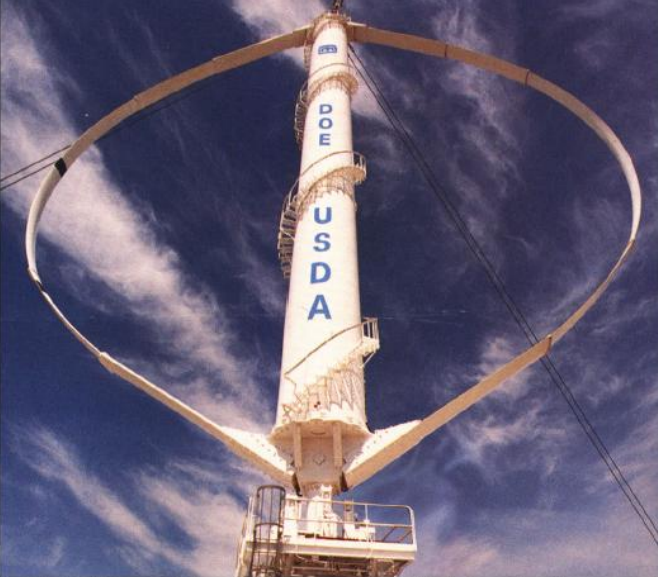
\includegraphics[width=\textwidth]{Murray2011-34m}

        \caption{Sandia 34 m diameter Test Bed, from \cite{Murray2011}.}

        \label{fig:Sandia-34m}
    \end{subfigure}
    \hfill
    \begin{subfigure}[b]{0.352\textwidth}
        \centering

        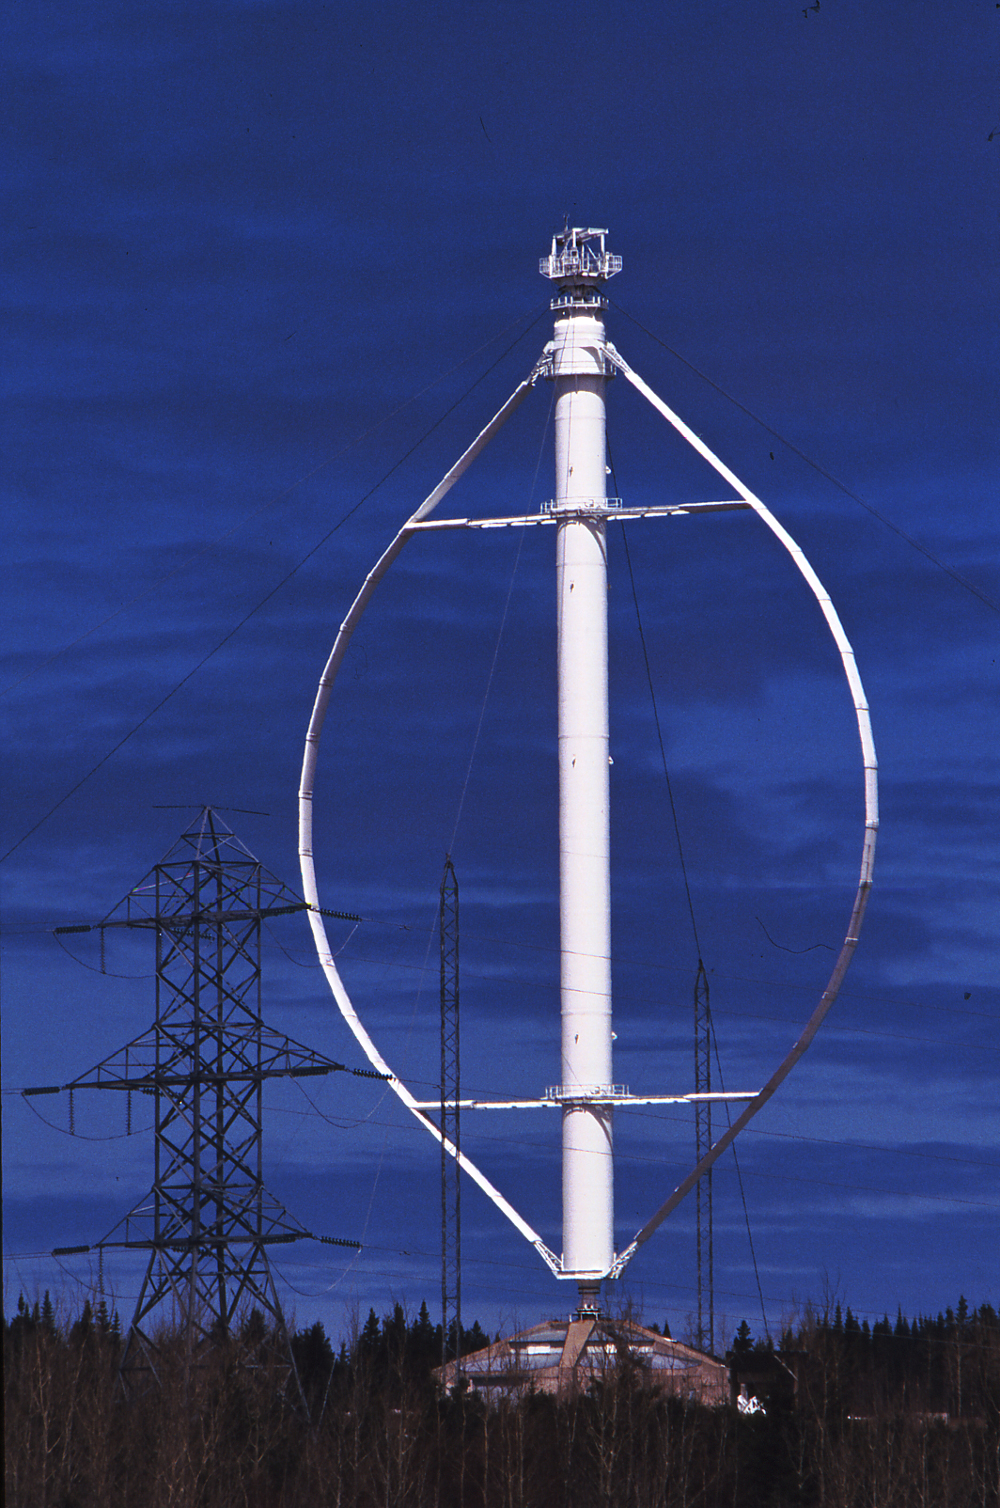
\includegraphics[clip, trim=0 0 0 0.05in, width=\textwidth]{Eole}

        \caption{Lavalin Eole 64 m diameter VAWT. Photo by Paul Gipe. All rights
            reserved.}

        \label{fig:Eole}
    \end{subfigure}

    \begin{subfigure}[b]{0.8\textwidth}
        \centering

        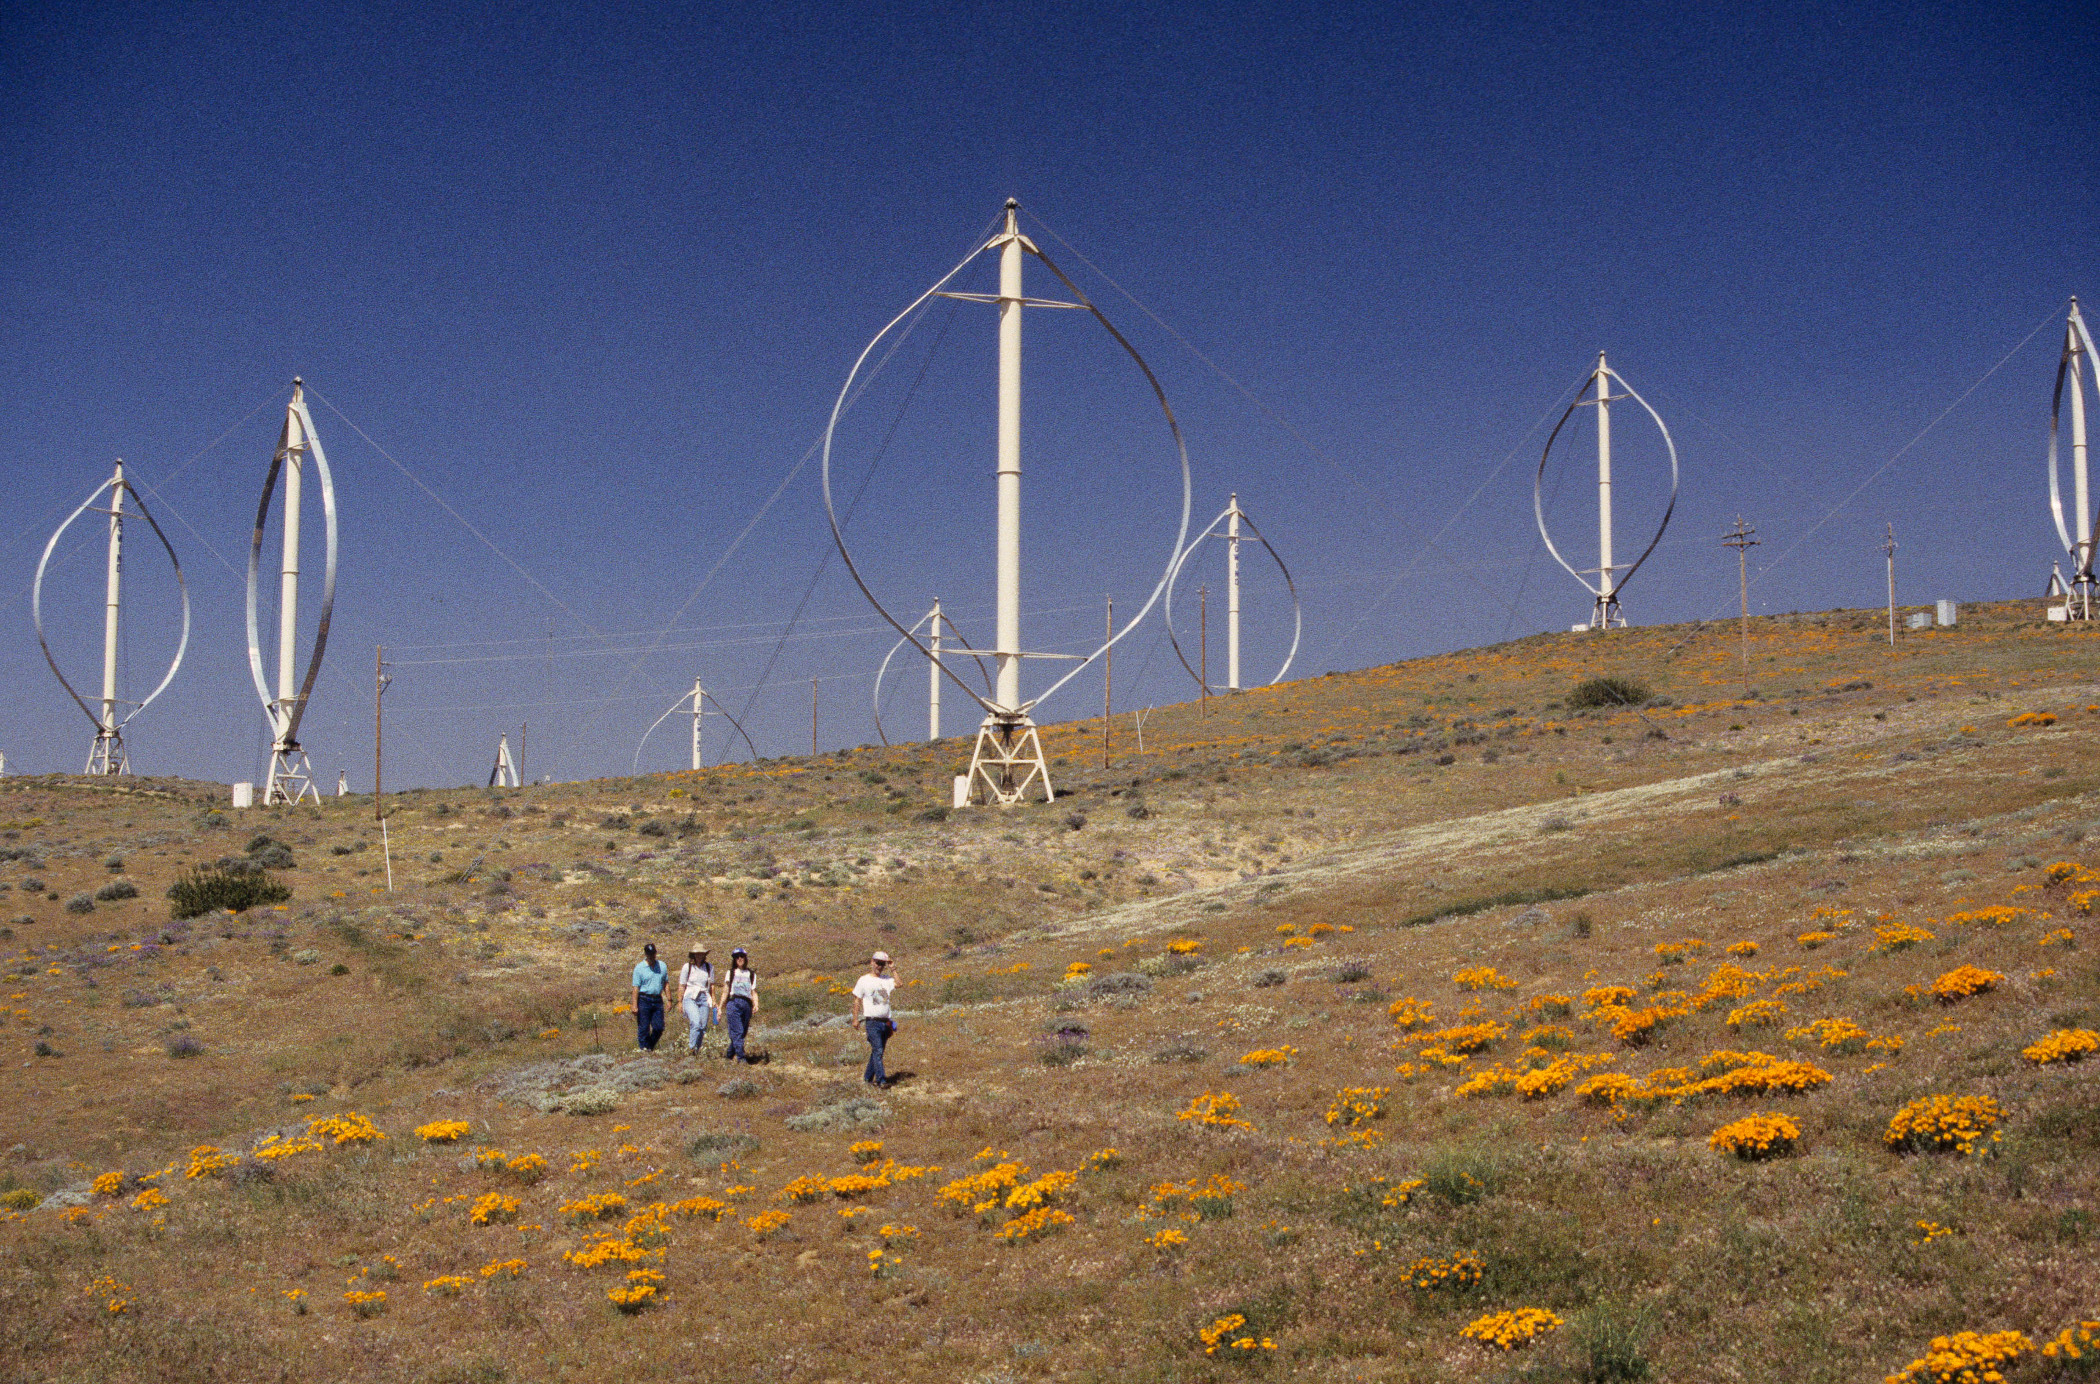
\includegraphics[width=\textwidth]{flowind}

        \caption{FloWind VAWT array. Photo by Paul Gipe. All rights reserved.}

        \label{fig:FloWind}
    \end{subfigure}

    \caption{Large scale Darrieus wind turbines: Sandia 34 m Test Bed (a),
        Lavalin Eole 64 m (b), and FloWind VAWT array (c).}

    \label{fig:Darrieus}
\end{figure}

Ultimately the three-bladed, horizontal-axis propeller-type axial-flow turbine
(AFT) concept---shown in Figure~\ref{fig:AFT} has became the design of choice
for large scale onshore wind---and for good reasons. Axial-flow turbines are
easier to analyze since their operating principle can essentially be idealized
as steady flow over a foil in an unstalled condition. AFTs also have the benefit
of research ``inertia''---a lot has been invested and a lot of knowledge has
accumulated already. As a result, the designs are quite mature, for wind energy
at least. In contrast, the CFT has been studied and applied significantly less,
though there have been cases where CFTs have performed nearly equally as well as
AFTs. However, CFTs are more difficult to design, since their blades are
continuously changing their angles of attack throughout the turbine's rotation,
often undergoing dynamic stall as part of normal operation \cite{Para2002},
which makes blade loading hard to predict. Beside their unpredictability, the
highly oscillatory blade loading presents significant design challenges for
avoiding fatigue---a main cause for failure or premature retirement of the large
Darrieus wind turbines.

\nomenclature{AFT}{Axial-flow turbine.}

\begin{figure}
    \centering

    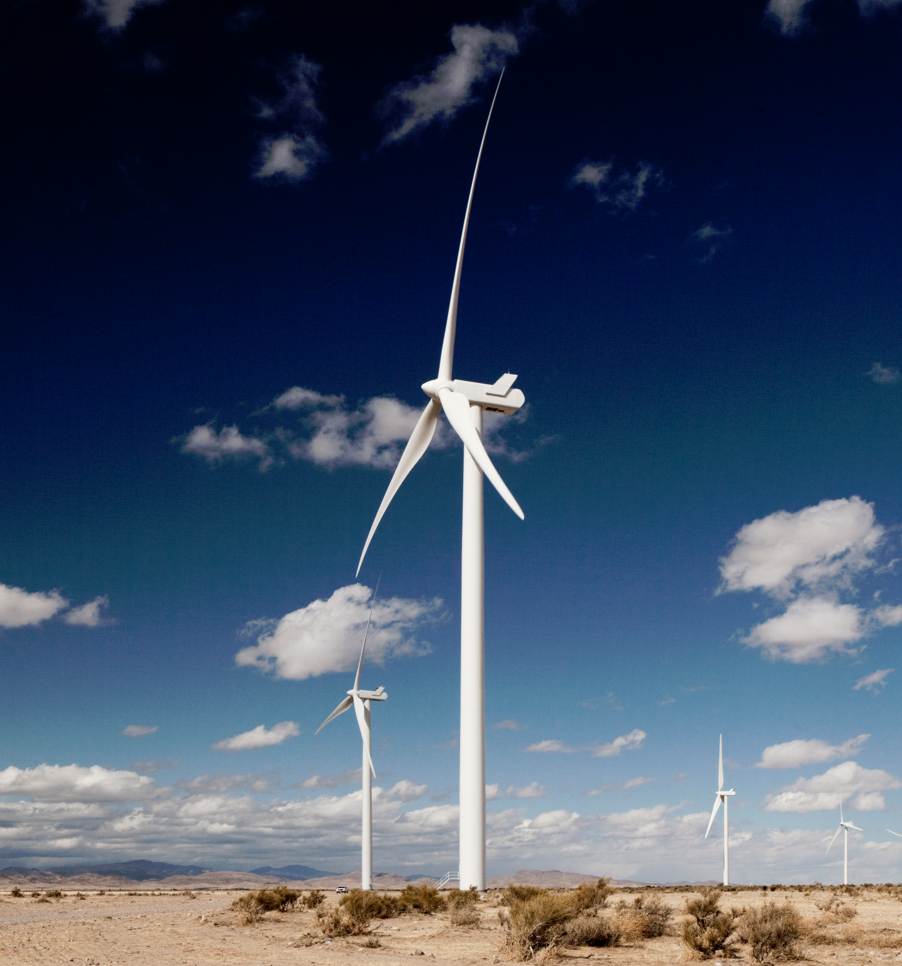
\includegraphics[width=0.7\textwidth]{Vestas-V100}

    \caption{Vestas V100 1.8 MW three-bladed axial-flow, a.k.a horizontal-axis
        wind turbine. Courtesy of Vestas Wind Systems A/S.}

    \label{fig:AFT}
\end{figure}

Despite these engineering challenges, CFTs may have advantages over AFTs under
certain conditions. They are simpler, omni-directional machines, which do not
require yawing or pitching mechanisms. There were considerations in the 2010s by
DEEPWIND in Europe \cite{Paulsen2011} and SNL \cite{Sandia2012} in the US for
using large scale floating VAWTs for offshore wind, since along with the
omni-directionality, a vertical shaft allows placement of the generator and
gearbox lower in the machine, which lowers center of gravity. In the onshore
wind arena, CFTs show promise for projects where space is limited, e.g., urban
environments, as adjacent turbines sometimes interact ``constructively'' to
increase each other's power outputs \cite{Li2010}---a trait not possessed by
AFTs. It has been claimed that arrays of VAWTs can potentially provide an
order-of-magnitude increase in the power output per land area of a wind turbine
array, since the devices can be spaced more closely than HAWTs
\cite{Dabiri2011}. Field measurements have shown that their wakes recover more
quickly than those of AFTs, and this cannot be entirely attributed to higher
turbulence generation \cite{Kinzel2012}. This phenomenon is investigated in
later chapters.

\nomenclature{VAWT}{Vertical-axis wind turbine.}

In the built, i.e., suburban and urban environments, wind resources are less
understood, more variable in terms of direction, speed, and turbulence levels
\cite{Smith2012}. Kooiman and Tullis \cite{Kooiman2010} observed that a
cross-flow turbine in an urban environment was indeed insensitive to changes in
wind direction, and was only adversely affected by temporal variations in wind
speed when turbulence intensity was above 15\%. The lack of need for yawing can
help lower cost of energy from CFTs versus AFTs by reducing complexity, e.g., by
eliminating slip rings. Cross-flow turbines may also have an advantage in the
urban environment since they must be designed for high fatigue loads anyway.
Recently, the Eiffel tower in Paris, France has been outfitted with two 5.3 m
tall, 3.2 m diameter helical vertical-axis cross-flow turbines, which will
produce at least 10 MWh/yr, or approximately 1 kW on average, which is expected
to power the entire first floor of the facility \cite{Lott2015}.

For MHK development, a field much less mature than wind power, the cross-flow
turbine concept is playing a major role thanks to its omni-directionality and
flexibility with respect to frontal area shape, allowing for more precisely
tuned fitment in channels with complex bathymetry or installed structures.
Chosen by the Ocean Renewable Power Company (ORPC) for their Turbine Generator
Unit (TGU), integrated as part of their TidGen system, a cross-flow turbine was
the first grid-connected tidal energy device in the US, which was installed in
Cobscook Bay, ME \cite{ORPC2012}. Today, ORPC is working on improving their
turbine's performance, and planning for the installation of 4 more turbines
\cite{Nelson2013}.

CFTs are also being considered for micropower applications, such as powering
remote underwater instrumentation packages that currently rely on batteries
\cite{Polagye2013b}. They are also being used in riverine applications, for
example, in ORPC's RivGen project in the Kvichak River just downstream of the
village of Igiugig, AK~\cite{Forbush2015}. Instream energy has also installed a
25 kW CFT in the Roza irrigation canal in Yakima, WA \cite{Gunawan2014}.

It could be argued that the failure of cross-flow turbines in the utility scale
onshore wind industry is the result of less-than-adequate predictive capability
in the engineering process. That is, issues such as lackluster performance and
fatigue could have been overcome. In order for modern cross-flow turbines to be
effective, these predictive or modeling capabilities must be enhanced, for both
individual devices and arrays, which is a primary motivation for this research.


\section{Principles of cross-flow turbine operation}

Blade element theory, originally conceived by
Drzewiecki~\cite{Drzewiecki1892,Drzewiecki1920}, is the analysis of a rotor or
propeller as a collection of 2-D foil sections, or blade elements, and can be
employed to obtain a simplified view of the kinematics and dynamics of a CFT.
Figure~\ref{fig:vectors} shows the relevant velocity and force vectors on a CFT
blade element. The relative velocity $U_{\mathrm{re}}$ and angle of attack
$\alpha$ are calculated by adding the inflow velocity vector $U_{\mathrm{in}}$
to the opposite of the blade element velocity $\omega r$, where $\omega$ is the
shaft angular velocity and $r$ is the element radius, which for a
straight-bladed turbine is equal to the maximum rotor radius $R$. In the
relative velocity coordinate system, the lift ($F_l$) and drag ($F_d$) forces
are then oriented normal and tangential to the relative velocity, respectively.
These forces, combined with the blade element pitching moment $M$ ultimately
produce the shaft torque, and in turn the shaft power.

\begin{figure}
    \centering

    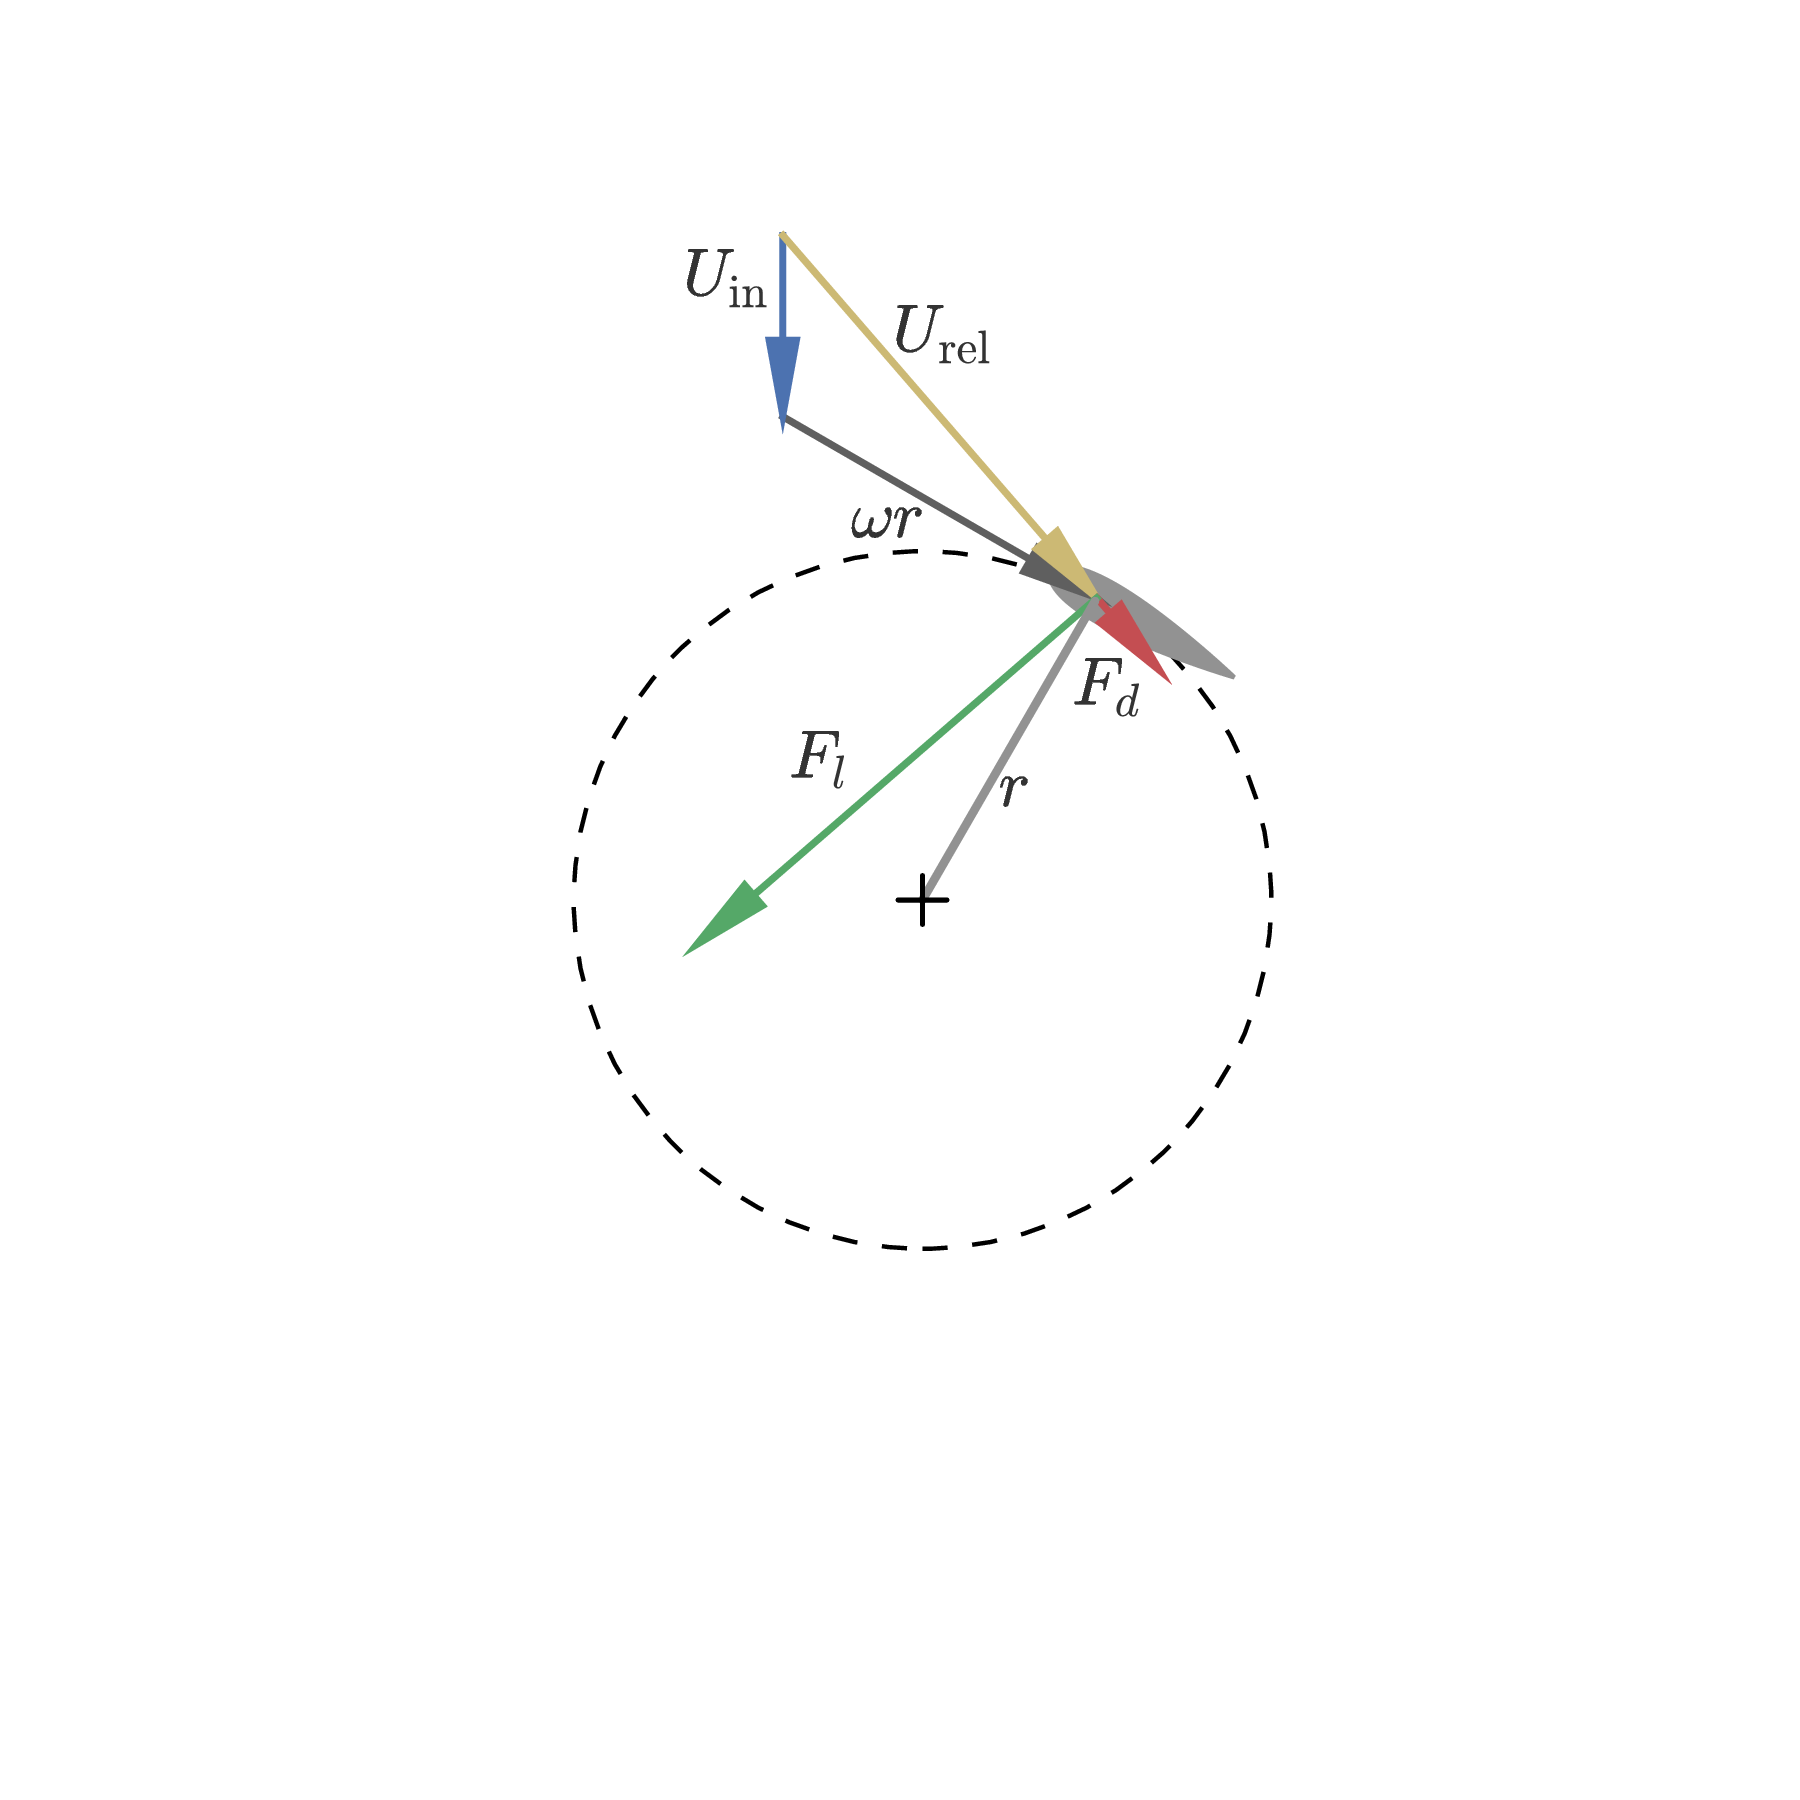
\includegraphics[clip, trim=1in 1.5in 1in 0.5in,
    width=0.5\textwidth]{figures/CFT-vectors_cft-vectors}

    \caption{Vector diagram of velocity and forcing on a cross-flow turbine
        blade element. Note that the free stream velocity $U_\infty$ is oriented
        from top to bottom (identical to $U_in$ for purely geometric calculations),
        the blade chord (dash-dotted line) is coincident with the tangential
        velocity (i.e., zero preset pitch, which would offset the geometric angle of
        attack $\alpha$), and the drag vector is magnified by a factor of two
        (approximately, relative to the lift vector) to enhance visibility.}

    \label{fig:vectors}
\end{figure}

The shaft's angular velocity $\omega$ is nondimensionalized as the tip speed
ratio
\begin{equation}
    \lambda = \frac{\omega R}{U_\infty},
    \label{eq:lambda}
\end{equation}
where $U_\infty$ is the free stream velocity. The turbine's shaft torque, $T$,
is characterized by the nondimensional torque coefficient
\begin{equation}
    C_T = \frac{T}{\frac{1}{2} \rho A R U_\infty^2},
    \label{eq:ct}
\end{equation}
where $\rho$ is the fluid density and $A$ is the turbine's frontal area.
Similarly, the turbine power $P = T\omega$ and overall rotor drag $F_D$ are
normalized as the power coefficient
\begin{equation}
    C_P = \frac{T \omega}{\frac{1}{2} \rho A U_\infty^3},
    \label{eq:cp}
\end{equation}
and the rotor drag (a.k.a. thrust) coefficient
\begin{equation}
    C_D = \frac{F_D}{\frac{1}{2} \rho A U_\infty^2}.
    \label{eq:cd}
\end{equation}
It is also worth noting that $C_P = \lambda C_T$.

\nomenclature{$\omega$}{Turbine shaft angular velocity.}
\nomenclature{$C_P$}{Turbine power coefficient.}
\nomenclature{$C_D$}{Overall rotor drag (or thrust) coefficient.}
\nomenclature{$C_T$}{Turbine torque coefficient.}
\nomenclature{$T$}{Shaft torque.}
\nomenclature{$\rho$}{Fluid density.}
\nomenclature{$A$}{Turbine frontal area.}
\nomenclature{$\lambda$}{Turbine tip speed ratio.}
\nomenclature{$R$}{Maximum rotor radius.}
\nomenclature{$U_\infty$}{Free stream velocity.}
\nomenclature{$C_m$}{Blade element pitching moment coefficient.}

So why then, is it so difficult to analyze these machines? A first glimpse can
be seen in Figure~\ref{fig:geom-alpha-urel}, where the geometric angle of attack
and relative velocity magnitude are plotted over one turbine revolution for
various tip speed ratios. Note that by considering geometry alone, we are
neglecting the effect of the blade element forcing on the local inflow velocity
vector---the so-called induction---which will most significantly decrease the
inflow and angle of attack on the downstream half of the blade path, i.e., for
$180 < \theta < 360$. If we imagine a typical high solidity $\sigma = Nc/R$
turbine, where $N$ is the number of blades, operating at an optimal tip speed
ratio $\lambda_0 = 2$, for example \cite{Howell2010} (note that solidity and
$\lambda_0$ are inversely correlated \cite{Templin1974}), we see that geometric
angles of attack can be very high even in optimal conditions.

\nomenclature{$\sigma$}{Turbine rotor solidity or ratio of total planform area
    to swept area.}
\nomenclature{$N$}{Number of blades.}
\nomenclature{$\lambda_0$}{Typical operating tip speed ratio, or that at which
    power coefficient is maximum.}

\begin{figure}
    \centering

    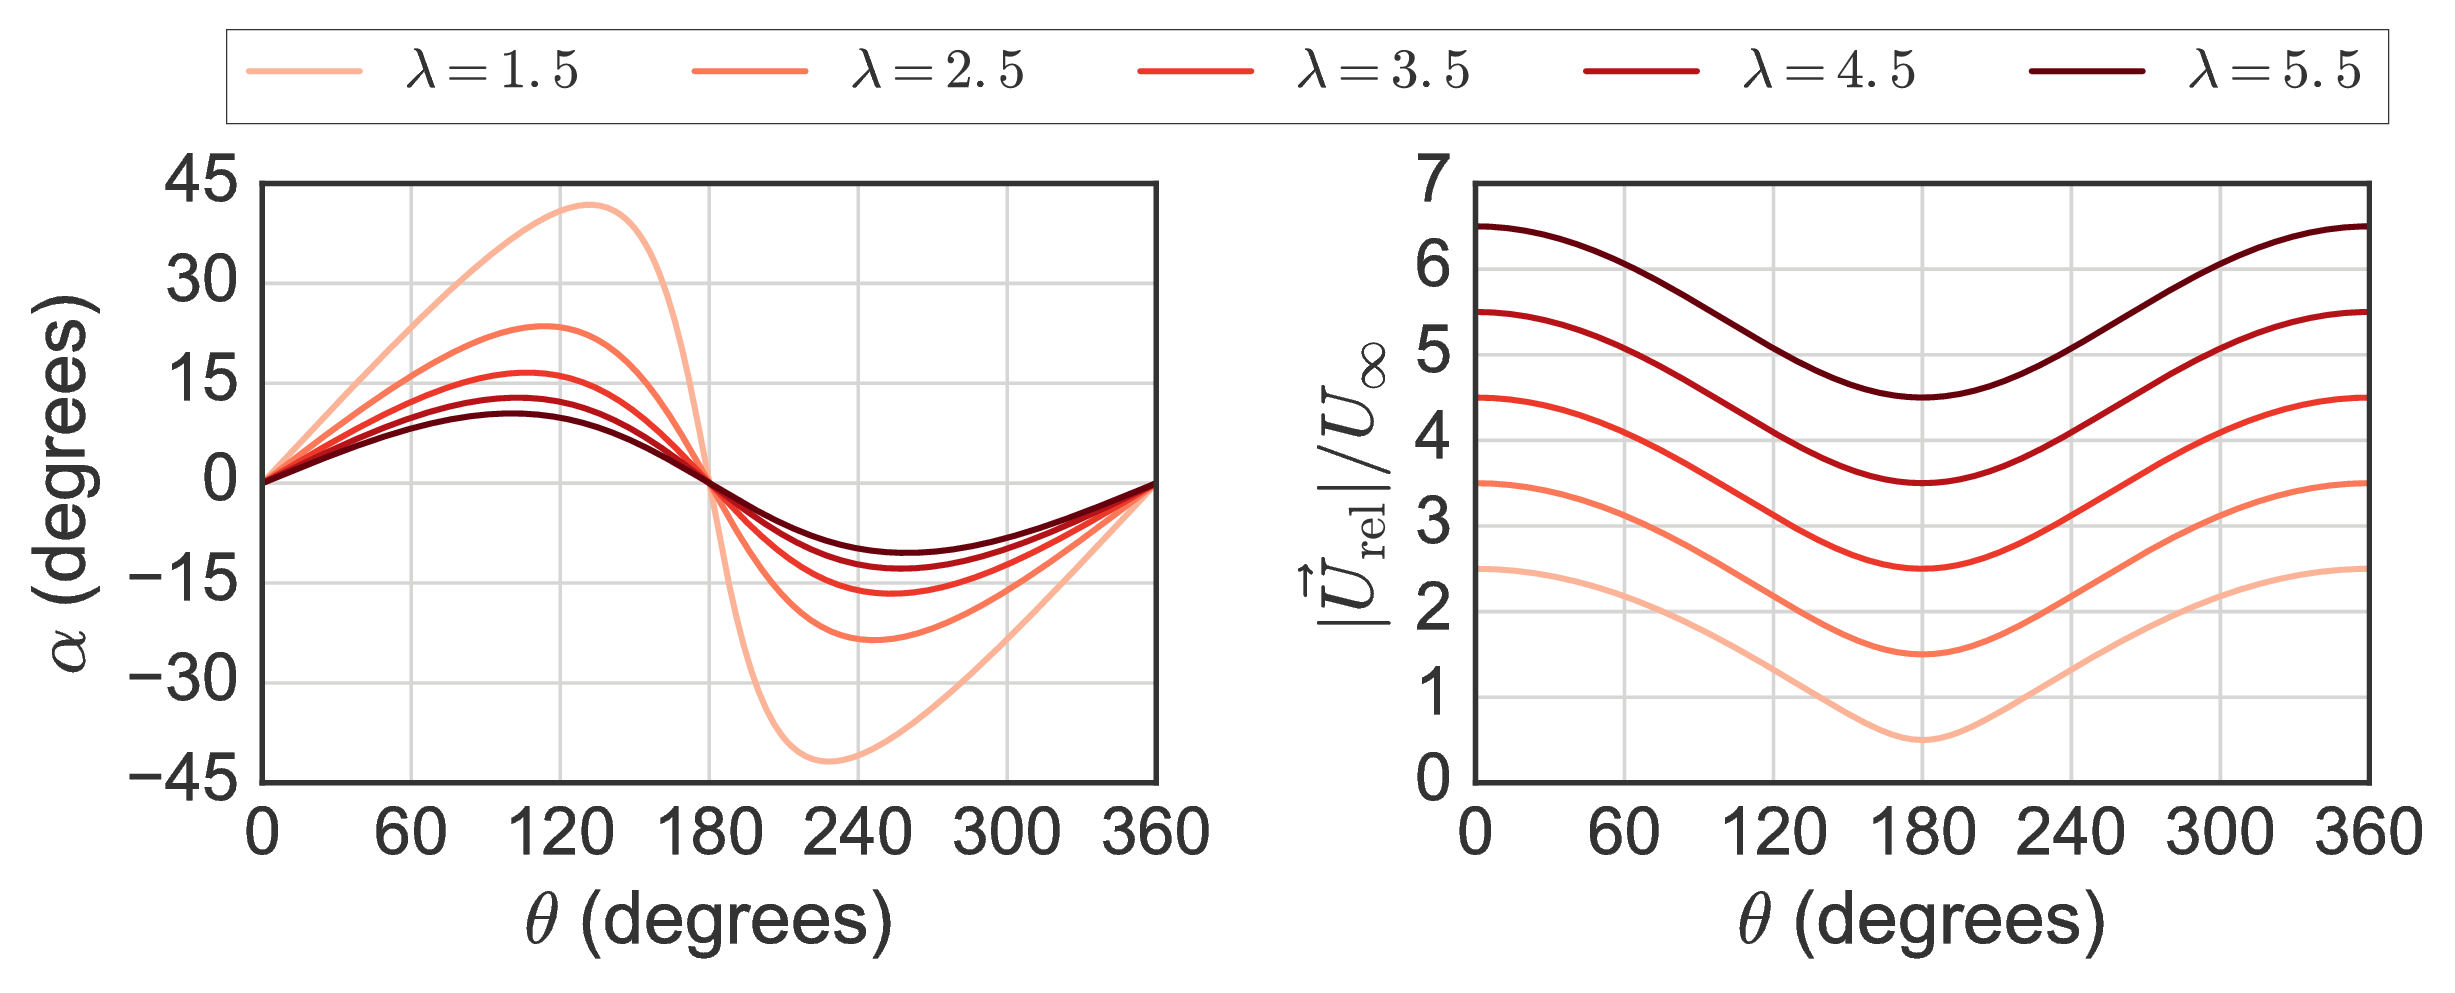
\includegraphics[width=0.85\textwidth]{CFT-vectors_alpha_deg_urel_geom}

    \caption{Geometric angle of attack (left) and relative velocity (right)
        versus azimuthal angle at various tip speed ratios.}

    \label{fig:geom-alpha-urel}
\end{figure}

As shown in Figure~\ref{fig:vectors}, the blade's lift to drag ratio and angle
of attack can be thought of as the quantities to maximize in order to develop
shaft torque. However, beyond a threshold angle of attack, i.e., the static
stall angle, $C_l/C_d$ drops. Predicting foil characteristics (lift, drag,
pitching moment) is difficult beyond the static stall angle, where boundary
layer separation becomes dominant over most of the foil suction surface, which
reduces lift and increases drag dramatically. For example,
Figure~\ref{fig:S826-perf} shows measured lift and drag coefficients for an S826
airfoil at $Re_c=145,000$ compared with 2-D and 3-D Navier--Stokes CFD
simulations from Cakmakcioglu et al. \cite{Cakmakcioglu2014}. The linear lift
slope region and static stall angle are predicted well enough, but the peak
$C_l/C_d$ is massively overestimated, due to both an overprediction of lift and
underprediction of drag. This may not be an issue for a machine designed to
operate at relatively fixed and/or pre-stall $\alpha$, e.g., airplane wings,
propellers, or axial-flow wind turbines, but a cross-flow turbine will most
likely encounter post-stall regimes, cf. Figure~\ref{fig:geom-alpha-urel},
making even high-fidelity CFD analysis an uncertain prospect for accurate blade
load prediction.

\nomenclature{$C_l$}{Foil or blade element lift coefficient.}
\nomenclature{$C_d$}{Foil or blade element drag coefficient.}
\nomenclature{$Re_c$}{Reynolds number based on chord length.}

\begin{figure}
    \centering

    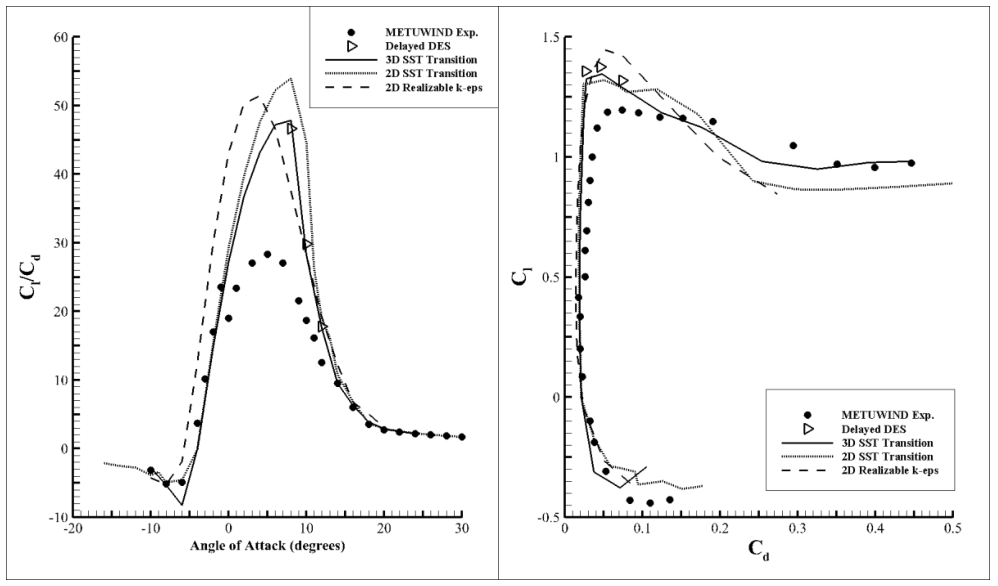
\includegraphics[width=\textwidth]{Cakmak-et-al-2014-fig8}

    \caption{Characteristics of an S826 airfoil at $Re_c=145,000$, from
        \cite{Cakmakcioglu2014}.}

    \label{fig:S826-perf}
\end{figure}


\subsection{Unsteady aerodynamics and dynamic stall}

Up until now we have only considered the static behavior of foils, which may be
sufficient to model the steady performance of an axial-flow turbine, since
angles of attack for all rotor blade elements are meant to remain constant in
ideal conditions. The rotation of a cross-flow turbine, however---with its
constantly changing angle of attack (also the change in sign) and relative
velocity---produces an unsteady environment for the blade elements, even in an
idealized case.

Unsteady foil behavior has been studied extensively in rotorcraft research
\cite{Leishman2006}. In the absence of stall, even a helicopter rotor airfoil
will deviate from static behavior due to cyclic pitching, along with changes in
relative velocity as the blade advances and retreats. Thus, the wealth of
knowledge available from the helicopter literature provides insight into the
cross-flow turbine case.

The first consideration is the attached behavior of unsteady airfoils. As one
might expect, in these cases either the angle of attack or relative velocity is
varying, but large amounts of flow separation, i.e., stall, is never
encountered. The unsteadiness is characterized by a reduced
frequency~\cite{Leishman2006}
\begin{equation}
    k = \frac{\omega c}{2 U_\infty},
\end{equation}
which assumes the free stream velocity is constant. Unsteady effects begin to
become significant for $k > 0.05$, and can become dominant for $k \ge
0.2$~\cite{Leishman2006}.

\nomenclature{$c$}{Foil or blade element chord.}

For a cross-flow turbine reduced frequency can be reformulated in terms of the
tip speed ratio as
\begin{equation}
    k = \frac{\lambda c}{2R},
\end{equation}
which is then also a function of solidity or chord-to-radius ratio $c/R$. As an
example, a large scale, relatively low solidity Darrieus turbine such as the
Sandia 34 m diameter Test Bed, with an equatorial blade chord of 0.91 m
\cite{Murray2011}, a reduced frequency $k=0.16$ is encountered based solely on
angle of attack oscillations at $\lambda=6$. For a smaller scale CFT, e.g., with
$c/R = 0.25$, operating at $\lambda = 2$, the reduced frequency is 0.25. It
follows that unsteady effects will be significant for cross-flow turbines even
in the absence of nonlinear effects such as stall.

In the unsteady regime, when a foil's angle of attack exceeds the static stall
angle, it encounters dynamic stall. The effects on foil loading are different
from those of static stall in that they are time dependent and include
hysteresis or lag effects. The dynamic stall process in general can be described
as \cite{McCroskey1981}, depicted in Figure~\ref{fig:McCroskey}:
\begin{enumerate}
    \item Attached flow with a thin boundary layer.

    \item Separation begins. A large leading edge vortex is formed, which causes
    an overshoot in lift beyond the static case in a linear fashion.

    \item The vortex is advected downstream, causing additional lift and
    negative pitching moment.

    \item The vortex advects towards the trailing edge. Lift and moment decay
    rapidly after reaching peak values.

    \item Secondary vortices may be shed, leading to additional lift and moment
    peaks.

    \item Forces slowly return to the linear regime as flow reattaches.
\end{enumerate}

\begin{figure}
    \centering

    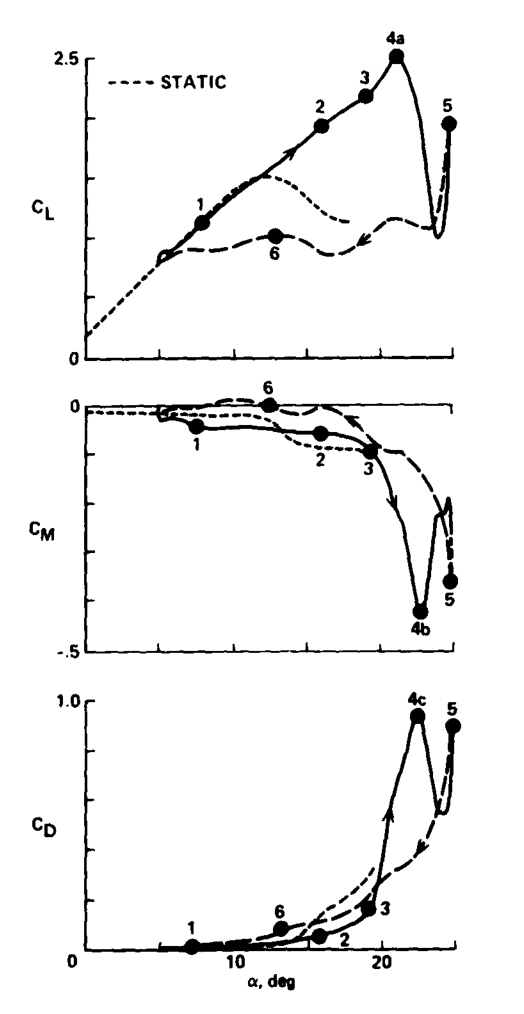
\includegraphics[height=0.9\textheight]{McCroskey-1981}

    \caption{Dynamic stall events for a Vertol VR-7 airfoil, taken from
        \cite{McCroskey1981}.}

    \label{fig:McCroskey}
\end{figure}

Based on Figure~\ref{fig:geom-alpha-urel}, we expect dynamic stall to play an
important role in governing overall blade loading for a cross-flow turbine.
Therefore, it is necessary to either accurately model dynamic stall, or employ
CFD methods that can resolve unsteady effects in the foil boundary layer, both
of which will be explored in later chapters.


\section{The state of engineering tools for CFTs}

\subsection{For individual devices}

Presently, the most reliable predictor of turbine performance is physical
modeling (building prototypes or copying existing designs that have been
field-tested), so long as important dynamical scales (Reynolds number, mainly)
are sufficiently matched. It has been shown that performance becomes essentially
Reynolds number independent at an approximate blade chord Reynolds number $Re_c
\approx \lambda U_\infty c / \nu = O(10^5)$ \cite{Bravo2007}, which is
investigated further in Chapter~\ref{chap:Re-dep}. However, experiments at this
scale can be quite expensive. For example, a turbine with a 1 m diameter and 10
cm chord would need to be tested in a flow on the order of 1 m/s in water and 10
m/s in air. For a turbine this large it is typically impractical to manufacture
many prototypes to find the optimal design, so numerical modeling is preferred.
There exists a large spectrum of numerical modeling techniques with widely
varying computational cost and fidelity, and sometimes only the most complex and
computationally expensive are trustworthy.

\nomenclature{$\nu$}{Fluid kinematic viscosity.}

Momentum models are the simplest and computationally least expensive, where the
turbine blades are discretized into blade elements, for which 2-D static lift
and drag data are tabulated. The relative velocity and angle of attack for a
blade element are calculated by seeking a balance between forces computed from
the static foil data and the rate of change of momentum of the fluid passing by
the blade element, computed within a single or multiple ``streamtubes.''
Momentum methods break down for large streamwise forces, i.e., ``induction
factors''---common in water and high solidity turbines---and must be corrected
empirically. Despite their deficiencies, these models can do a reasonable job
for low solidity rotors when combined with corrections for dynamic loading, the
most prominent cause of which is dynamic stall \cite{Para2002}, but fail for
high solidity~\cite{Joo2015}. A double multiple streamtube (DMST) momentum model
can compute a full turbine performance curve in seconds on a modern desktop
computer.

\nomenclature{DMST}{Double multiple streamtube.}

Vortex line methods are similar to momentum models, except blade element local
velocity is computed using potential flow theory, where lifting bodies are bound
vortex lines that shed vortex wake elements whose influences are combined via
the Biot--Savart law \cite{Strickland1979}. Sandia National Labs' CACTUS is one
example of a vortex line code \cite{Murray2011}. CACTUS has been tested against
experimental data from large, low-solidity wind turbines (those for which
momentum models do well), but has been shown to fail for smaller turbines in
water, which are typically higher solidity \cite{Michelen2014}. Regarding
computing effort, vortex line methods can compute a full turbine performance
curve for a simple geometry in minutes---longer than the DMS method, but still
quite fast. However, in some cases vortex methods can become quite expensive,
e.g., when turbines contain many bound vortex elements, and/or the simulation
must be run for long times, where the number of shed vortices becomes large. The
increase in accuracy of the flow field prediction and the robustness with
respect to high turbine loading justify the slightly higher expense of the
vortex line method.

A more sophisticated vortex model is the so-called panel method, where turbine
geometry can be specified arbitrarily as potential flow boundary elements,
negating the need for sectional foil coefficient tables. This is a significantly
more computationally expensive model---see for example~\cite{Dixon2008}---in
spite of its increased generality. Furthermore, boundary layer models are
necessary to predict the occurrence and consequences of dynamic
stall~\cite{Zanon2012}, and since the fluid dynamics are still assumed to be
governed by potential flow, effects of turbulence are not resolved.

The most computationally expensive models solve the Navier--Stokes equations,
with turbulence modeled with Reynolds-averaging (RANS) or large eddy simulation
(LES)---the former being relatively less expensive, since LES directly solves a
larger portion of the energy spectrum of turbulence. If a body-fitted grid is
used, the actual turbine geometry is included as part of the computational
domain, and the mesh is generally refined next to the solid surfaces to resolve
the boundary layer, i.e., with cells adjacent to walls having a nondimensional
wall distance $y^+ = u^* y / \nu \sim 1$, where $u^*$ is the friction velocity,
defined as $u^*=\sqrt{\tau_w / \rho}$, where $\tau_w$ is the wall shear stress.
When only run in two dimensions, RANS methods are affordable enough to be run on
a single CPU, computing a single turbine operating point in hours. However, 3-D
effects are important enough that 2-D simulations are not reliable, at least as
predictors of absolute performance \cite{Li2013}. 3-D simulations with a
body-fitted grid are very expensive (especially for LES), therefore are
practically limited to high performance computing (HPC) clusters. Even with the
high computational expense, these models are not perfect and results can deviate
significantly from experimental measurements, especially when using RANS models
\cite{Li2013}.

\nomenclature{$y^+$}{Nondimensional wall distance.}
\nomenclature{$u^*$}{Friction velocity.}
\nomenclature{$\tau_w$}{Wall shear stress.}
\nomenclature{LES}{Large eddy simulation.}

Actuator line modeling (ALM), first used by Sorensen and
Shen~\cite{Sorensen2002}, is a hybrid of the blade element and Navier--Stokes
methods. The turbine is not part of the mesh, but is represented by lines that
move through the flow, acting as momentum sinks, where the resultant force is
computed using 2-D foil data. Negating the needs for a body-fitted grid and
resolving the boundary layer removes a significant amount of computational
effort, but the flow field is still computed more accurately than with momentum
or vortex methods, since nonlinear effects and turbulence are included in the
RANS or LES equations. Removing the need for complex grids is also an advantage
with respect to  mesh generation, which is arguably the largest impediment to
automation in CFD \cite{Slotnick2014}. Computational effort is also
significantly reduced since the ALM does not need a rotating mesh.

\nomenclature{ALM}{Actuator line model.}
\nomenclature{CFD}{Computational fluid dynamics.}
\nomenclature{RANS}{Reynolds-averaged Navier--Stokes.}

To the author's knowledge, at the time of
this writing there has only been one study in the literature investigating the
ALM for CFTs \cite{Shamsoddin2014}, which was performed for a 2-D rotor at very
low Reynolds number, for which performance predictions were not reported.
Assessing its effectiveness is therefore of interest in the present work.


\subsection{For arrays}

Effective turbine array engineering directly depends on accurate prediction of
turbine wake generation, evolution and interaction, along with the impact of
various types of turbulent inflow on power production of each device. Like for
individual turbines, physical modeling is an option for predicting array
performance, though it becomes even more expensive to match relevant dynamical
scales. For this reason, turbine arrays are mainly designed using numerical
methods.

The contemporary industry standard method for predicting array performance
involves the superposition of prescribed wakes \cite{Stevens2014b}. Evolution
can be dependent on a single expansion coefficient chosen by the free stream
turbulence intensity \cite{Jensen1983, Choi2013} or computed by a solution of
the linearized RANS equations with an empirically derived constant eddy
viscosity closure \cite{Ainslie1988}. While these models may be acceptable for
analyzing HAWT farms, in light of the CFT's unique near-wake dynamics, the
validity of these models for application to CFT arrays is questionable. At the
very least they would need to be recalibrated for CFTs, though their
applicability is limited in the near-wake of any turbine, meaning they are
generally inappropriate for closely-spaced arrays.

\nomenclature{HAWT}{Horizontal-axis wind turbine.}
\nomenclature{CFT}{Cross-flow turbine.}

The next step up in complexity is the actuator disk method, where a constant
body force is added to the Navier--Stokes equations. This method can be
computationally cheap with RANS, or quite expensive and thorough with LES. The
ORPC turbine array in Cobscook Bay, Maine is being laid out using the SNL-EFDC
code, which uses a constant uniform force applied to the RANS equations, where
the turbine injects turbulence kinetic energy and dissipation for the model's
$k$--$\epsilon$ closure \cite{Nelson2013}. The ability of actuator disk models
to predict the near-wakes of CFTs is of interest in this work.

At present simulations with body-fitted grids are limited to one or two turbines
due to computational cost, which means they are impractical for full array
simulations. Thus the actuator line method, when combined with LES, is the most
complex model being used today. The ALM has the benefit of resolving unsteady
flow features created by periodic blade forcing and end effects, ultimately
producing the most accurate parameterization for turbine induced forces in
Navier--Stokes simulations. It has been shown in blind axial-flow turbine
modeling tests that ALM/LES methods fair better when predicting turbine induced
turbulence, and therefore will be more accurate at predicting flow within a
turbine array \cite{Krogstad2013}.


\section{Goals and objectives}

At the most basic level, the goal this research is to work towards the ability
to predict the performance of and flow though an array of cross-flow turbines,
to allow for the evaluation of array layouts, and the prediction of overall
power output and potential environmental effects. The strategy for meeting this
goal includes the following objectives:

\begin{enumerate}
	\item To improve the understanding of both high and low solidity cross-flow
    turbine wakes, most importantly the apparent increased rate of momentum and
    energy recovery compared with axial-flow turbines. This will establish our flow
    modeling targets.

    \begin{enumerate}
        \item To evaluate the ability of actuator disk models to predict the
        wakes of cross-flow turbines.
    \end{enumerate}

	\item To assess the allowable scale mismatch at which physical models can
	provide results relevant to full-scale devices and arrays.

	\item To evaluate the ability of high-fidelity blade-resolved computational
    fluid dynamics and high performance computing to supplement or possibly replace
    experimental work.

    \item To investigate actuator line modeling to potentially reduce the
    required computing power necessary for engineering work with CFTs.
\end{enumerate}

An additional overarching goal is to release all research products---data, code,
CAD models, simulation case files---as openly as possible to enable
reproducibility and maximize reuse.


\section{Contributions to science and engineering}

Cross-flow turbines are simple machines made from common shapes, i.e., foils,
but they can produce very complex flows. Despite their failure in the large
scale wind industry, and beyond their contemporary adoption in marine
hydrokinetics, there is scientific and engineering value to better understanding
their behavior. The flow problem---unsteady foil behavior involving dynamic
stall, finite blade span end effects in curvilinear flows---is complex yet
general enough to be applicable to other unsteady turbomachinery and/or foil
flows, e.g., Voith Schneider propellers, Cyclogyros, or even conventional
helicopter rotors.

The experiments performed as part of this work have helped elucidate the unique
wake features of cross-flow turbines~\cite{Bachant2015-JoT} and establish
scaling guidelines for physical modeling and numerical model
validation~\cite{Bachant2016-Energies}. This is especially important for CFTs
since typical designs for small wind and MHK use have not yet been established.
This means that in order to be robust, numerical models must be tested against
measurements from turbines with varying design parameters, notably the solidity
and aspect ratio, which affect the unsteadiness and significance of 3-D effects,
respectively. There is a danger that validating against the most ubiquitous
Darrieus turbine experiments may result in models that fail with newer, more
unique designs.

In addition to conventional publications, the datasets collected and analyzed
have been provided openly \cite{Bachant2014-RVAT-baseline,
    Bachant2016-RVAT-Re-dep, Bachant2016-RM2-data}, both for a high and
low-to-medium solidity turbine. These datasets will help others evaluate their
numerical models, and since their availability also includes processing code,
other researchers may find new knowledge to glean from them.

Lastly, the effectiveness of state-of-the-art Navier--Stokes based numerical
modeling techniques was evaluated, and an actuator line model was developed and
validated against performance and wake measurements for three-dimensional
cross-flow turbines operating at Reynolds numbers relevant to full scale.
Software tools here have also been made open-source, e.g.,
\cite{Bachant2016-turbinesFoam-v0.0.7}, have been made available to the public
throughout all phases of development, and have benefited from open collaboration
as well.
